\chapter{Distribución $ \Gamma $ (Gamma) }
Este modelo es una generalización del modelo \textit{exponencial}.

\section{Descripción}
Se utiliza para modelar  variables que describen el tiempo hasta que se produce p veces un determinado suceso. \cite{wiki:3}

\section{PDF}
\begin{center}
	$ f(x) = \frac{\beta^\alpha}{\Gamma(\alpha)} x^{\alpha - 1} e^{\beta x}$
\end{center}

\subsection{Parámetros}
Los parámetros observables son:

\begin{center}
	\begin{tabular} {| l | l |}
		\hline
		$\alpha$ & shape parameter\\ \hline
		$\beta$ & shape parameter\\ \hline		
	\end{tabular}
\end{center}

\section{CDF}
\begin{center}
	$ f(X < x) = \frac{1}{\Gamma(\alpha)} \gamma{\alpha, \beta x}$
\end{center}

\section{MGF}
\begin{center}
	$ m = (1 - \frac{t}{\beta})^{\alpha}$
\end{center}
\section{Media y Varianza}
\subsection{Media}
\begin{center}
	$E(x) = \frac{\alpha}{\beta}$
\end{center}

\subsection{Varianza}
\begin{center}
	$Var(x) = \frac{\alpha}{\beta^2}$
\end{center}

\section{Gráficas}

\begin{center}
	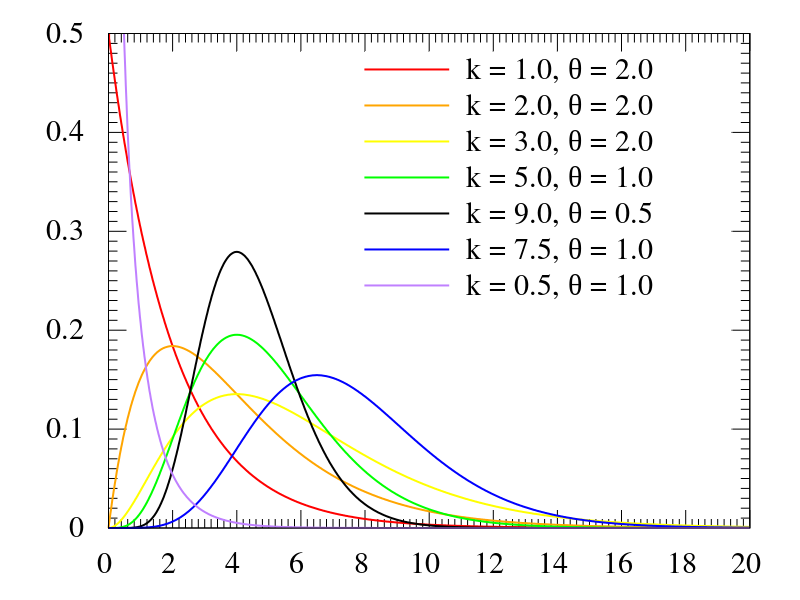
\includegraphics[scale=0.5]{imgs/gamma-pdf.png}
	
	\textit{PDF}
\end{center}

\begin{center}
	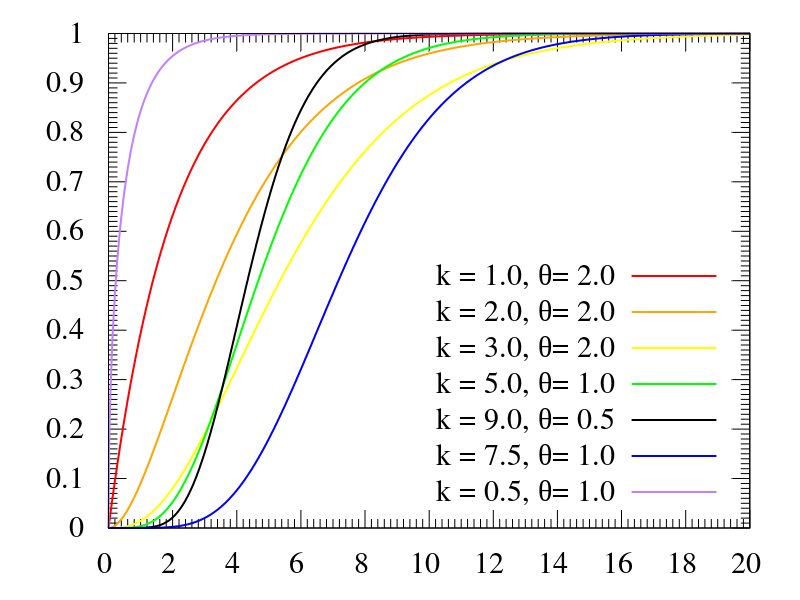
\includegraphics[scale=0.5]{imgs/gamma-cdf.png}
	
	\textit{CDF}
\end{center}

\section{Aplicaciones en la vida real}
Comunmente es usado para determinar el tiempo necesario para observar eventos en un intervalo definido.

Por ejemplo: Edad para contraer matrimonio, tiempo de fallas de sistemas...
